\def\b#1{\mathbf{#1}}


\subsection{Binární vyhledávací stromy, vyvažování, haldy}

\subsubsection*{Binární strom}

\begin{definice}
\emph{Dynamická množina} je množina prvků (datová struktura), měnící se v čase. Každý její prvek je přístupný přes ukazatel a obsahuje:
\begin{pitemize}
    \item \emph{klíč} (jednu položku, typicky hodnotu z lin. uspořádané množiny), 
    \item \emph{ukazatel(e)} na další prvky, 
    \item případně \emph{další data}.
\end{pitemize}
Na takové množině jsou definovány tyto operace:
\begin{pitemize}
    \item \emph{find} - nalezení prvku podle klíče
    \item \emph{insert} - přidání dalšího prvku
    \item \emph{delete} - odstranění prvku
    \item \emph{min}, \emph{max} - nalezení největšího / nejmenšího prvku
    \item \emph{succ}, \emph{pred} - nalezení následujícího / předcházejícího prvku k nějakému předem danému
\end{pitemize}
\end{definice}


\begin{definice}
\emph{Binární strom} je dynamická množina, kde každý prvek (uzel, node) má kromě klíče a příp. dalších dat tři ukazatele na \emph{levého} a \emph{pravého} syna a rodiče. Speciální uzel je \emph{kořen}, který má NULLový ukazatel na rodiče. Ten je v binárním stromě jeden. Uzly, které mají NULLové ukazatele na pravého i levého syna, se nazývají \emph{listy}.

\emph{Podstrom} je část stromu (vybrané prvky), která je sama stromem - např. pokud se jako kořen určí jeden z prvků. \emph{Levý(pravý)} podstrom nějakého prvku je strom, ve kterém je kořenem levý(pravý) syn tohoto prvku. \emph{Výška stromu} je délka nejdelší cesty od kořenu k listu.
\end{definice}

Binární strom je \emph{vyvážený}, pokud max. 1 uzel má jednoho syna (tj. všechny vnitřní uzly kromě až na jeden mají oba syny, listy z definice nemají žádného). Výška vyváženého stromu roste logaritmicky vzhledem k počtu uzlů. Výška nevyváženého stromu může růst až lineárně vzhledem k počtu prvků (i \uv{spojový seznam} je platný bin. strom).


\subsubsection*{Binární vyhledávací strom}

\begin{definice}
\emph{Binární vyhledávací strom} je takový binární strom, ve kterém je jeho struktura určená podle klíču jeho uzlů: pro každý uzel s klíčem hodnoty $k$ platí, že jeho levý podstrom obsahuje jen uzly s menší hodnotou klíče než $k$ a jeho pravý podstrom jen uzly s hodnotou klíče větší nebo rovnou $k$.
\end{definice}

\begin{algoritmusN}{Vyhledávání v bin. stromě}
\begin{verbatim}
Find( x - kořen, k - hledaná hodnota klíče ){
  while( x != NULL && k != x->klíč ){
    if ( k < x->klíč )
      x = x->levý_syn;
    else
      x = x->pravý_syn;
  }
  return x;
}
\end{verbatim}

Složitost je $O(h)$ v nejhorším případě, kde $h$ je výška stromu (tj. pro nevyvážené stromy až $O(n)$ kde $n$ je počet prvků). Asymptotická časová složitost ostatních operací je stejná.

Vložení a vymazání prvku se provádí prostým nalezením místa, kam by se prvek měl vložit (nebo kde už je), a přepojením pointerů.
\end{algoritmusN}

\subsubsection*{Vyvažované vyhledávací stromy}

Kvůli zajištění větší rychlosti (menší asymptotické časové složitosti) operací byly vytvořeny speciální druhy binárních vyhledávacích stromů, které jsou průběžně vyvažovány, aby měly max. výšku menší než $c\cdot\log n$, kde $n$ je počet uzlů a $c$ nějaká konstanta.

\begin{definiceN}{Pomocné operace na stromech}
Pro vyvažování stromů při vkládání a odebírání uzlů se definují pomocné operace: \emph{pravá} a \emph{levá rotace}. Zachovávají vlastnosti bin. vyhledávacích stromů a jsou proveditelné v konstatním čase - jde jen o přepojení uzlů násl. způsobem (pro pravou rotaci na uzlu $Q$ a levou na $P$):

\begin{center}
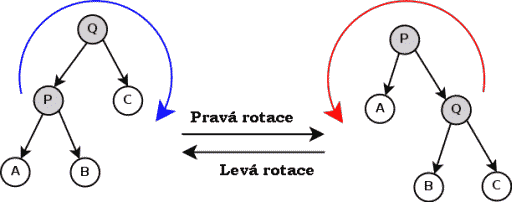
\includegraphics[width=12cm]{informatika/algoritmy_a_ds/obrazky/tree_rotation.png}

(Zdroj obrázku: Wikipedia)
\end{center}
\end{definiceN}


\begin{definiceN}{Červeno-černé stromy}
Červeno-černé stromy jsou binární vyhledávací stromy s garantovanou max. výškou $O(\log n)$, kde $n$ je počet uzlů, tj. operace na nich mohou mít asymptotickou časovou složitost $O(\log n)$. Pro jejich popis je nutné definovat \emph{interní uzly} - všechny uzly stromu a \emph{externí uzly} - na (interních) listech (a uzlech s jedním potomkem) uměle přidané NULLové ukazatele (de facto \uv{listy} červeno-černého stromu). Externí uzly slouží jenom jako abstrakce pro popis stromů, při implementaci se s nimi neoperuje. Červeno-černý strom má tyto čtyři povinné vlastnosti:
\begin{penumerate}
    \item Každý uzel (externí i interní) má definovanou barvu, a to černou nebo červenou.
    \item Každý externí uzel je černý.
    \item Každý červený vrchol musí mít oba syny černé.
    \item Každá cesta od libovolného vrcholu k listům v jeho podstromě musí obsahovat stejný počet černých uzlů.
\end{penumerate}

Pro červeno-černé stromy se definuje \emph{výška uzlu} $x$ ($\b{h}(x)$) jako počet uzlů na nedelší možné cestě k listu v jeho podstromě. \emph{Černá výška uzlu} ($\b{bh}(x)$) je počet černých uzlů na takové cestě.
\end{definiceN}

\begin{vetaN}{Vlastnosti červeno-černých stromů}
Podstrom libovolného uzlu $x$ obsahuje alespoň $2^{\b{bh}(x)}-1$ interních uzlů. Díky tomu má červeno-černý strom výšku vždy nejvýše $2\log(n+1)$ (kde $n$ je počet uzlů). (Důkaz prvního tvrzení indukcí podle $\b{h}(x)$, druhého z prvního a třetí vlastnosti červeno-černých stromů)
    \end{vetaN}

\begin{dusledek}
Operace hledání (minima, maxima, následníka, \dots), které jsou stejné jako u obecných binárních vyhledávacích stromů, mají garantovanou časovou složitost $O(\log n)$.
\end{dusledek}

\begin{algoritmusN}{Vkládání a odebírání uzlů v červeno černých stromech}
Obě operace mají podle garantované max. výšky garantovanou čas. složitost $O(\log n)$ pro $n$ počet uzlů. Protože bez porušení vlastností červeno-černých stromů lze kořen vždy přebarvit načerno, můžeme pro ně předpokládat, že \emph{kořen stromu} je \emph{vždy černý}.

\emph{Vkládání} vypadá následovně:
\begin{pitemize}
    \item Nalezení místa pro vložení a přidání nového prvku jako v obecných bin. vyhl. stromech, nový prvek se přebarví načerveno.
    \item Pokud je jeho otec černý, můžeme skončit -- vlastnosti stromů jsou splněné. Pokud je červený, musíme strom upravovat (tady předpokládám, že otec přidávaného uzlu je levým synem, opačný připad je symetrický):
    \item Je-li i strýc červený, přebarvit otce a strýce načerno a přenést chybu o patro výš (je-li děd černý, končím, jinak můžu pokračovat až do kořene, který už lze přebarvovat beztrestně).
    \item Je-li strýc černý a přidaný uzel je levým synem, udělat pravou rotaci na dědovi a přebarvit uzly tak, aby odpovídaly vlastnostem stromů.
    \item Je-li strýc černý a přidaný uzel je pravým synem, udělat levou rotaci na otci a převést tak na předchozí případ.
\end{pitemize}

\emph{Odebírání} se provádí takto:
\begin{pitemize}
    \item Odstraním uzel stejně jako v předchozím případě. Opravdu odstraněný uzel (z přepojování) má max. jednoho syna. Pokud odstraňovaný uzel byl červený, neporuším vlastnosti stromů, stejně tak pokud jeho syn byl červený -- to řeším jeho přebarvením načerno.
    \item V opačném případě (tj. syn odebíraného -- $x$ -- je černý) musím udělat násl. úpravy (přep. že $x$ je levým synem svého nového otce, v op. případě postupuji symetricky):
    \item $x$ prohlásím za \uv{dvojitě černý} a této vlastnosti se pokouším zbavit.
    \item Pokud je bratr $x$ (buď $w$) červený, pak má 2 černé syny -- provedu levou rotaci na rodiči $x$, prohodím barvy rodiče $x$ a uzlu $w$ a převedu tak situaci na jeden z násl. případů:
    \item Je-li $w$ černý a má-li 2 černé syny, prohlásím $x$ za černý a přebarvím $w$ načerveno, rodiče přebarvím buď na černo (a končím) nebo na \uv{dvojitě černou} a propaguji chybu (mohu dojít až do kořene, který lze přebarovat beztrestně).
    \item Je-li $w$ černý, jeho levý syn červený a pravý černý, vyměním barvy $w$ s jeho levým synem a na $w$ použiji pravou rotaci, čímž dostanu poslední případ:
    \item Je-li $w$ černý a jeho pravý syn červený, přebarvím pravého syna načerno, odstraním dvojitě černou z $x$, provedu levou rotaci na $w$ a pokud měl původně $w$ (a $x$) červeného otce, přebarvím $w$ načerveno a tohoto (teď už levého syna $w$) přebarvím načerno.
\end{pitemize}
\end{algoritmusN}


\begin{definiceN}{AVL stromy (Adelson-Velsky \& Landis)}
\emph{AVL stromy} jsou, podobně jako červeno-černé stromy, bin. vyhledávací stromy, které zaručují max. logaritmický nárůst výšky vzhledem k počtu prvků. Pro každý uzel $x$ se v AVL stromu definuje \emph{faktor vyvážení} jako rozdíl výšky jeho levého a pravého podstromu: $\b{bf}(x) = h(\texttt{x->levý}) - h(\texttt{x->pravý})$. Pro všechny uzly v AVL stromu platí, že $|\b{bf}(x)|\leq 1$.
\end{definiceN}

\begin{vetaN}{Zaručení výšky AVL stromů}
Výška AVL stromu s $n$ vrcholy je $O(\log n)$. (Důkaz: buď $T_n$ AVL strom výšky $n$ s minimálním počtem uzlů. Ten má podstromy $T_{n-1}$ a $T_{n-2}$ atd., tj. velikost minimálního AVL stromu roste jako Fibonacciho posloupnost, tedy $|T_n|\geq (\frac{1+\sqrt{5}}{2})^{n-1}$. Důkaz tohoto indukcí.)
\end{vetaN}

\begin{algoritmusN}{Operace na AVL stromech}
Vyhledávací operace se provádí stejně jako na obecných bin. vyhledávacích stromech, vkládání a odebírání prvků taky, ale pokud tyto operace poruší zákl. vlastnost AVL stromů ($|\b{bf}(x)=2|$), je nutné provést vyvažování -- pomocí rotací (které mohou být propagovány až ke kořeni). Při vkládání a odebírání je navíc nutné průběžně (nejhůře až ke kořeni) upravovat indikaci faktoru vyvážení jednotlivých uzlů.
\end{algoritmusN}

\subsubsection*{Halda}

\begin{definice}
\emph{Halda(heap)} je dynamická množina se stromovou strukturou (binární halda je binární strom), pro kterou platí tzv. \uv{vlastnost haldy}: $$\text{ Je-li }x\text{ potomek }y\text{, pak }x\texttt{->klíč}\geq y\texttt{->klíč}$$ Haldy s touto nerovností jsou tzv. \emph{min-heap}y, pokud je nerovnost opačná, jde o \emph{max-heap}.
\end{definice}

\begin{obecne}{(Binární) haldy}
Binární haldy jsou nejčastějším typem haldy. Zajišťují nalezení minimálního prvku v konstantním čase a odebrání a přidání minima v čase $O(\log n)$. V každé hladině od první až do předposlední je max. možný počet uzlů, v poslední jsou uzly co nejvíce \uv{vlevo} -- tedy max. výška haldy s $n$ prvky je $(\log n) + 1$. Proto je pro binární haldy jednoduše proveditelná jejich datová reprezentace polem (bez pointerů), kde při indexování od 0 má uzel na indexu $k$:
\begin{pitemize}
    \item Levého a pravého syna na indexu $2k+1$, resp. $2k+2$ (pokud to není víc než celk. počet prvků, potom syny nemá).
    \item Rodiče na indexu $\lceil\frac{k}{2}\rceil-1$. 
\end{pitemize}

\emph{Přidání uzlu} do haldy znamená přidání prvku na konec haldy a dokud má jeho rodič větší klíč, jeho prohazování s rodičem (tedy posouvání o vrstvu výš). Při \emph{odebírání uzlu} z haldy tento nahradím posledním prvkem v haldě a potom dokud neplatí vlastnost haldy (nejméně jeden z potomků má menší klíč), prohazuji ho s potomkem s menším klíčem (a posouvám o vrstvu níž).

Vytvoření haldy je možné v čase $O(n)$, kde $n$ je počet prvků v haldě -- přidání 1 prvku do haldy trvá $O(h)$, kde $h$ je aktuální výška (a $h$ roste od $0$ až k $\lceil\log n\rceil$, počet prvků ve výšce $k$ je $\frac{n}{2^{k+1}}$, bereme-li výšku listů rovnou nule) - v součtu za všechny prvky jde o $O(n\cdot\sum_{h=0}^{\lceil\log n\rceil}\frac{h}{2^h})$.

Binární halda se používá např. k \emph{třídění haldou} (heapsortu), kdy se z dat, která je potřeba utřídit, nejdříve postaví halda, a potom se opakuje operace odebrání kořene (tj. minimálního prvku).
\end{obecne}

\begin{obecne}{Fibonacciho haldy}
Fibonacciho haldy mají nízkou časovou složitost běžných operací -- amortizovaně $O(1)$ pro vložení, hledání minima apod.; odebrání prvku a odebrání minima má složitost $O(\log n)$ pro $n$ prvků v haldě. Tvoří ji skupina stromů, vyhovujících \uv{vlastnosti haldy}. Každý uzel haldy s $n$ prvky má max. $\log n$ potomků a ve svém podstromě minimálně $F_{k+2}$ uzlů, kde $F_k$ je $k$-té Fibonacciho číslo. To je zajištěno pravidlem, že při odebírání prvků lze z nekořenového uzlu oddělit max. 1 syna, jinak je nutné oddělit i tento uzel a ten se pak stane kořenem dalšího stromu. Počet stromů se snižuje při odebírání minima, kdy jsou spojovány dohromady.

Fibonacciho haldy se používají pro efektivní implementaci složitějších operací, jako např. Jarníkova nebo Dijkstrova algoritmu.
\end{obecne}
